\usetikzlibrary{calc,arrows.meta}
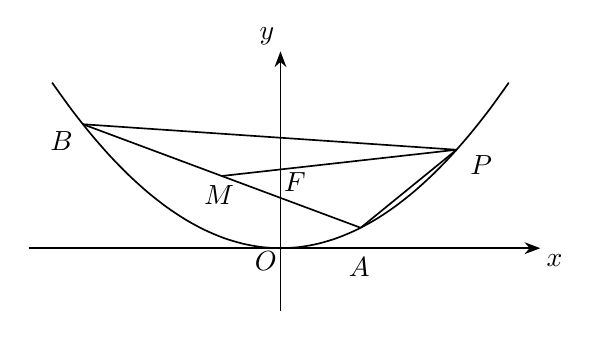
\begin{tikzpicture}[x=1cm,y=1cm,line width=.6pt,font=\normalsize,>=Stealth]
\coordinate (O) at (0,0);
\coordinate (F) at (0,1);
\coordinate (A) at (1.0185,0.2593);
\coordinate (B) at (-2.5092,1.5740);
\coordinate (M) at (-0.7454,0.9167);
\coordinate (P) at (2.2361,1.25);
\draw[domain=-2.9:2.9,smooth,variable=\t] plot (\t,{0.25*\t*\t});
\draw[->] (-3.2,0)--(3.3,0) node[anchor=north west,inner sep=0pt,xshift=2pt,yshift=-2pt] {$x$};
\draw[->] (0,-0.8)--(0,2.5) node[anchor=south east,inner sep=0pt,xshift=-2pt,yshift=2pt] {$y$};
\draw (B)--(A);
\draw (P)--(B);
\draw (P)--(A);
\draw (P)--(M);
\node[below left,inner sep=1pt] at (O) {$O$};
\node[below right,inner sep=1pt] at (F) {$F$};
\node[inner sep=1pt] at (-0.78,0.68) {$M$};
\node[inner sep=1pt] at (1.00,-0.24) {$A$};
\node[inner sep=1pt] at (-2.78,1.36) {$B$};
\node[inner sep=1pt] at (2.55,1.05) {$P$};
\end{tikzpicture}
